%%%% CAPÍTULO — DESENVOLVIMENTO DO SISTEMA
%%
%% Corpo principal da monografia (TCC~2): o que foi feito no E-Museu.
%% Alinhar seções aos objetivos específicos e às evidências do repositório
%% (PRs, issues, wiki, deploy). Redigir em tempo verbal passado.

\chapter{Desenvolvimento do Sistema}\label{cap:desenvolvimento}

Este capítulo apresenta o desenvolvimento realizado na refatoração e na expansão do sistema web do E-Museu, desde o planejamento até a entrega operacional na \acrshort{utfpr}.


\section{Levantamento de requisitos e priorização}\label{sec:dev-requisitos}

O levantamento de requisitos constituiu a primeira etapa do trabalho. Os requisitos foram identificados principalmente a partir das observações da orientadora Dra. Sediane Carmem Lunardi Hernandes, que apontou, no sistema E-Museu, a necessidade de aprimoramentos na estrutura do código, bem como a ausência de testes automatizados, evidenciando a demanda por refatoração e pelo desenvolvimento de novas funcionalidades.

Após discussões e alinhamentos, os requisitos receberam ajustes a partir das contribuições do coorientador Dr. Diego Marczal e dos professores Me. Dênis Lucas Silva e Dr. Emerson André Fedechen, especialmente durante a primeira banca, o que permitiu um refinamento mais preciso e alinhado aos objetivos centrais do trabalho.

Com os requisitos definidos, foi aplicada a técnica de priorização MoSCoW, com o objetivo de direcionar o desenvolvimento para as funcionalidades de maior impacto no sistema, otimizando o uso do tempo, esforço e recursos disponíveis. O resultado dessa priorização é apresentado na Figura~\ref{fig:moscow}.

\begin{figure}[H]
    \centering
    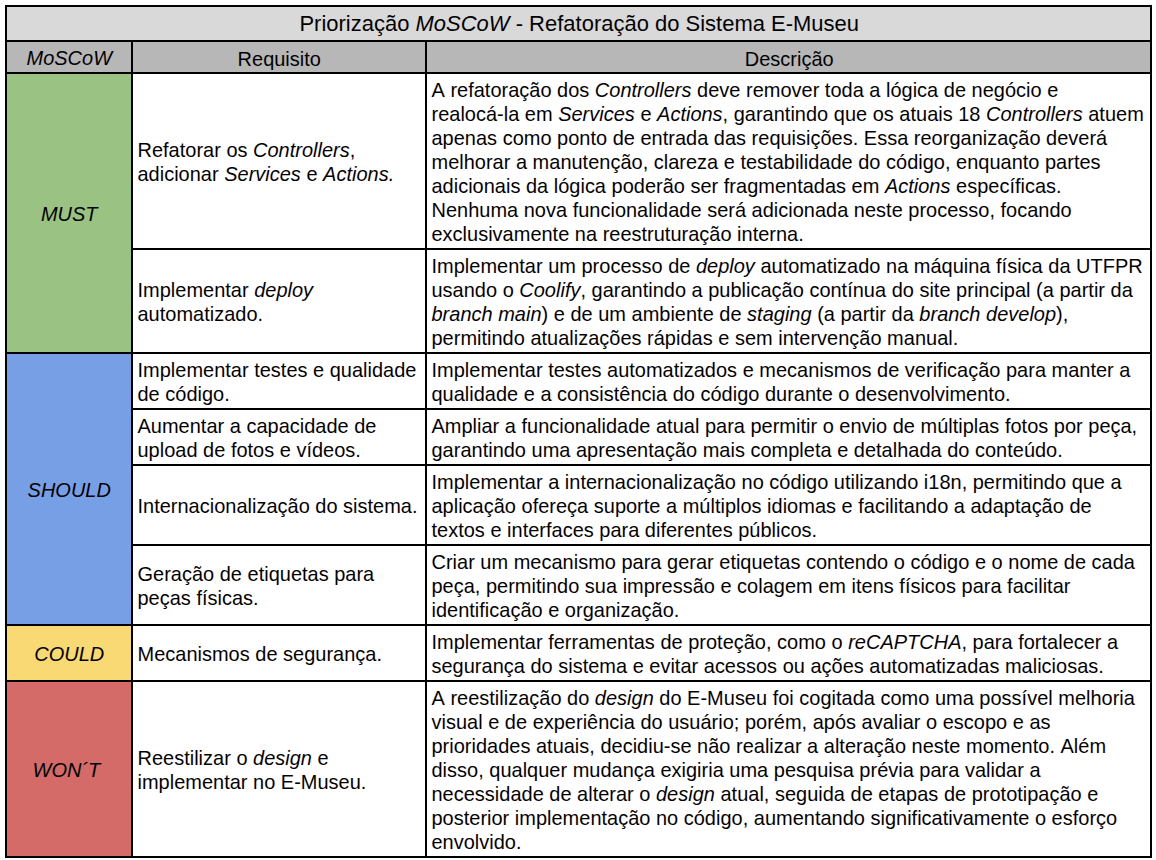
\includegraphics[width=\textwidth]{figuras/moscow.png}
    \caption{Priorização \acrshort{moscow}.}
    \label{fig:moscow}
    \caption*{\textbf{Fonte:} Autoria própria.}
\end{figure}


\section{Organização do repositório e fluxo de desenvolvimento}\label{sec:dev-gitflow}

\subsection{Documentação do Gitflow e convenções}

Para garantir um fluxo de desenvolvimento consistente e devidamente documentado, foi realizada, previamente ao início da implementação, uma elaboração completa da documentação referente ao Gitflow, convenções de \textit{commits}, gestão de \textit{issues} e demais práticas relacionadas ao versionamento. Toda essa documentação está disponível no repositório oficial do projeto \cite{gitflowdoc}.

% TODO: descrever perfil *full* (branches @dev/…, templates de PR/issue, labels).

\subsection{Criação do repositório e versionamento}

O repositório do E-Museu foi criado a partir de um \textit{fork}, que se trata de uma cópia independente de um projeto existente, permitindo sua evolução de forma separada da primeira versão desenvolvida por \cite{gonzaga2024}. A partir dele, estruturou-se uma configuração inicial de ambiente utilizando Docker Compose, servindo como base para o desenvolvimento posterior \cite{emuseurepo}.

% TODO: síntese do histórico de PRs/issues relevantes (sem depender de links externos no corpo).


\section{Configuração de ambientes e infraestrutura}\label{sec:dev-infra}

% TODO: Docker Compose local; ambientes staging e produção;
% Coolify na VM UTFPR; domínios staging.e-museu… e e-museu.gp.utfpr.edu.br;
% serviços auxiliares (MySQL, Redis, MinIO) quando aplicável.


\section{Refatoração da aplicação}\label{sec:dev-refatoracao}

% TODO: atualização Laravel/PHP; reorganização de controllers, services e actions;
% padrões MVC e boas práticas citados no referencial; exemplos pontuais (figuras ou trechos em apêndice).


\section{Testes automatizados e qualidade de código}\label{sec:dev-testes}

% TODO: linters, testes de fluxo/integração/usabilidade conforme objetivos;
% ferramentas adotadas e cobertura alcançada (valores a confirmar pelo autor).


\section{Funcionalidades implementadas}\label{sec:dev-funcionalidades}

% TODO, alinhado aos objetivos específicos:
% - upload múltiplo de fotos e link de vídeo;
% - internacionalização;
% - reCAPTCHA e segurança;
% - geração de etiquetas para peças físicas;
% - demais entregas priorizadas no MoSCoW.


\section{Implantação, validação e entrega institucional}\label{sec:dev-deploy}

% TODO: ciclo staging → produção; testes em ambiente controlado;
% pacote de continuidade (dump, backups, documentação operacional) entregue à UTFPR,
% sem expor credenciais no texto.


\section{Síntese dos resultados alcançados}\label{sec:dev-sintese-resultados}

Ao término das etapas descritas neste capítulo, consolidam-se os principais resultados do trabalho em relação ao objetivo geral (Seção~\ref{subsec:objetivoGeral}) e aos objetivos específicos (Seção~\ref{subsec:objetivoEspecificos}). A Tabela~\ref{tab:objetivos-resultados} resume, de forma sintética, o atendimento a cada meta e indica onde a evidência correspondente é detalhada no texto. Itens marcados como parciais ou não atendidos são discutidos nas limitações e nos trabalhos futuros (Seções~\ref{sec:conclusao-limitacoes} e~\ref{sec:conclusao-trabalhos-futuros}).

\begin{table}[H]
    \centering
    \caption{Síntese dos objetivos específicos e dos resultados alcançados.}
    \label{tab:objetivos-resultados}
    \begin{tabularx}{\textwidth}{@{}p{0.36\textwidth}Xp{0.14\textwidth}@{}}
        \toprule
        \textbf{Objetivo específico} & \textbf{Principal evidência no trabalho} & \textbf{Situação} \\
        \midrule
        Versionamento e padrões no GitHub &
        Seções~\ref{sec:dev-gitflow} e~\ref{sec:dev-requisitos} &
        % TODO: Atendido / Parcial / Não atendido
        a confirmar \\
        Ambientes de desenvolvimento, teste e produção &
        Seções~\ref{sec:dev-infra} e~\ref{sec:dev-deploy} &
        a confirmar \\
        Refatoração do código existente &
        Seção~\ref{sec:dev-refatoracao} &
        a confirmar \\
        Testes automatizados &
        Seção~\ref{sec:dev-testes} &
        a confirmar \\
        Novas funcionalidades do E-Museu &
        Seção~\ref{sec:dev-funcionalidades} &
        a confirmar \\
        Padrões de projeto e boas práticas &
        Seções~\ref{sec:dev-refatoracao} e~\ref{sec:dev-funcionalidades}; Capítulo~\ref{cap-referencial-teorico} &
        a confirmar \\
        \bottomrule
    \end{tabularx}
    \caption*{\textbf{Fonte:} Autoria própria. \textbf{Nota:} Preencher a coluna ``Situação'' após fechar o capítulo (por exemplo: atendido, parcial ou não abordado neste TCC).}
\end{table}

% TODO: parágrafo fechando: sistema em produção (e-museu.gp.utfpr.edu.br), comparação
% sucinta com a versão de \citeonline{gonzaga2024} e principais ganhos mensuráveis
% (ex.: ambientes separados, documentação de fluxo, quantidade de testes — confirmar números).

